

\documentclass[12pt,a4paper]{report}
\usepackage{graphicx}
\usepackage[utf8]{inputenc}
\usepackage[T1]{fontenc}
\usepackage[a4paper,top=3cm,bottom=2cm,left=3cm,right=3cm,marginparwidth=1.75cm]{geometry}
\usepackage[spanish]{babel}
\selectlanguage{spanish}
\usepackage{fancyhdr}

% quitar el 0.
\renewcommand\thesection{\arabic{section}}

% aqui definimos el encabezado de las paginas pares e impares.
\lhead[x1]{
\includegraphics[width=1cm]{./images/epis}}
\chead[y1]{}
\rhead[z1]{Inteligencia de Negocios}
\renewcommand{\headrulewidth}{1pt}

% aqui definimos el pie de pagina de las paginas pares e impares.
\lfoot[a1]{Ing. Patric Cuadros}
\cfoot[c1]{}
\rfoot[e1]{\thepage}
\renewcommand{\footrulewidth}{1pt}

\pagestyle{fancy} 



\begin{document}
\begin{titlepage}
	\centering
	
\includegraphics[width=4cm]{./images/upt}\par\vspace{1cm}
	{\scshape\LARGE\huge\bfseries Universidad Privada de Tacna \par}
	{\scshape\LARGE Escuela de Ingenieria de Sistemas \par}
	\vspace{1cm}
	{\scshape\Large Inteligencia de Negocios\par}
	\vspace{0.5cm}
	{\huge\bfseries Business Intelligence vs Business Analytics \par}
	\vspace{1cm}

	{\Large\itshape PRESENTADO POR:\par}
	{\Large\itshape Aldo Lopez Mamani\par}


	\vfill
	Docente\par
	Ing. Patrick Cuadros\textsc{Brown}

	\vfill

% Bottom of the page
	{\large \today\par}

\end{titlepage}

%% Aquí podemos añadir un resumen del trabajo (o del artículo en su caso) 
\begin{abstract}
\centering
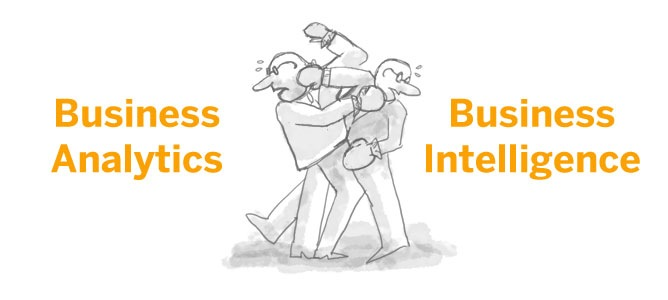
\includegraphics[width=14cm]{./images/foto2}\par\vspace{10cm}
\end{abstract}

%% Iniciamos "secciones" que servirán como subtítulos
%% Nota que hay otra manera de añadir acentos


\addcontentsline{toc}{chapter}{Índice general}
\tableofcontents
\newpage

\begin{Large}
\textbf{BIA VS BI} 
\end{Large}
\section{Business Inteligencie}
El concepto ‘Business Intelligence’, o inteligencia empresarial, se refiere al uso de datos en una empresa para facilitar la toma de decisiones. Es un conjunto de estrategias y herramientas enfocadas al análisis de datos de una empresa mediante el análisis de datos existentes.

Todas las empresas pueden recopilar datos, ya sean datos relativos a ventas, a compras, a inversiones, a tiempos, etc. Miles de datos y variables pueden ser estudiados y utilizados para tomar nuevas estrategias, conocer las fortalezas propias, y por supuesto, las debilidades. Todo lo que nos sea de utilidad para conocer nuestra empresa en profundidad y poder seguir mejorando. Este comportamiento de medición constante y análisis de los resultados es clave para alcanzar nuestros objetivos en el tiempo establecido. 

En términos generales, el Business Intelligence trata de extraer los datos de la empresa de distintas fuentes mediante las herramientas o técnicas ELT (extraer, cargar y transformar), o actualmente ETL (extraer, transformar y cargar), para luego cargarlos en un almacén de datos. Todo este análisis, debería permitir incrementar el nivel financiero, administrativo, y con las decisiones a mejorar las acciones de la empresa.

\subsection{Herramientas y soluciones de Business Intelligence}
En cuanto a las herramientas y metodologías de Business Intelligence, tienen algunas características comunes:
\begin{itemize}
\item Accesibilidad a la información. Sin información, sin datos, no hay nada que estudiar. Estas herramientas y técnicas garantizan el acceso a los datos por parte de los usuarios.
\item Apoyo en toma de decisiones. Acceso a herramientas de análisis que permitan a los usuarios seleccionar y manipular aquellos datos que les interesen.
\item Orientación al usuario final. Se busca independencia entre los conocimientos técnicos de los usuarios y su capacidad para utilizar estas herramientas.
\end{itemize}

En resumen, podremos decir que el Business Intelligence trata de personas que utilizan la tecnología para tomar decisiones. Y gracias a la tecnología, hoy día podemos conseguir muchos datos confiables sobre la empresa, desde ventas, hasta producción, pasando por gasto de combustible, kilómetros recorridos, gasto energético, y un largo etcétera de variables, que nos permitirán analizar unos hechos constatados, para valorar qué es susceptible de ser mejorado, cambiado, modificado, para obtener una mejora sustancial.

Es cierto que las soluciones tradicionales de Business Intelligence son difíciles de implantar, de mantener, de evolucionar y de usar, pero no en vano la tecnología avanza y nos está automatizando muchos procesos, y hay que invertir en esta tecnología (software y hardware), para mejorar los procesos. Pongamos algunos ejemplos. Podemos confiar en que un operario, repartidor de paquetería, cada día nos traiga su ruta, y kilómetros recorridos, comprobar su veracidad con el contador del vehículo y gasolina consumida e insertar esos datos en una base de datos. O mediante GPS y software, podemos hacer que la base de datos coja automáticamente el recorrido real del vehículo, distancia recorrida, consumo medio, y todo se calculará automático. Este gesto reduce el tiempo de recopilación de datos. Lo mismo podría aplicarse al tiempo de trabajo productivo realizado, listados de tareas finalizadas cada mes, etc.

Podríamos decir que sería trasladar a todos los apartados de la empresa algo que los departamentos financieros llevan haciendo con el dinero toda la vida. Datos que serán analizados, y servirán para realizar previsiones económicas a medio o largo plazo, y así tomar decisiones en todos los ámbitos. Por supuesto, son datos muy útiles también los indicadores de productividad, que nos permitirán realizar una serie de mejoras en los procesos de producción.

\section{Business Analytics}
BA es una expresión general para los enfoques y las tecnologías que puede utilizar para acceder y explorar los datos de su empresa, con el fin de extraer nuevos conocimientos útiles para mejorar la planificación empresarial y aumentar el rendimiento futuro.

Por lo general, esto implica el uso de análisis estadísticos y modelos predictivos para establecer tendencias, comprender por qué están sucediendo las cosas y hacer una idea aproximada de cómo se desarrollarán las cosas en el futuro.

Podemos entender Business Analytics como el conjunto de herramientas que ayudan en la toma de decisiones en todos los niveles de la empresa. Ayudando a las empresas a comprender mejor los resultados de negocio, a anticiparse a ellos y a darles forma mediante la habilidad de identificar tendencias, modelos y anomalías y analizarlos; comparar los casos “what-if” y predecir las amenazas y oportunidades potenciales; y planificar, presupuestar y prever los recursos.

Estudios recientes demuestran que las empresas que aplican la analítica obtienen unos resultados mejores que los de sus iguales. Y aquellas organizaciones con un alto Cociente Analítico es decir, con una filosofía general basada en analítica, tienen un rendimiento medio tres veces superior. La analítica de negocio permite que su organización identifique las tendencias y los patrones sutiles de modo que pueda anticiparse y controlar los acontecimientos para mejorar los resultados.

\begin{itemize}
\item Tome decisiones adecuadas y optimizadas en cualquier momento y lugar, para mejorar sus resultados y controlar el riesgo. Entre las aplicaciones en Business Analytics destacan:
\item  Business Intelligence. Conectar a las personas con la información cuándo, dónde y cómo lo necesiten, y colabore para mejorar el rendimiento de negocio.
\item  Rendimiento financiero y gestión estratégica. Dirigir la estrategia de gestión hacia los objetivos más rentables mediante información fiable y puntual y la creación de informes transparente y oportuna.
\item Analítica predictiva. Identificar patrones y asociaciones sutiles y desarrollar modelos predictivos para optimizar la toma de decisiones.
\item  Gobierno, riesgo y cumplimiento normativo. Obtener un mayor conocimiento en todos los aspectos relacionados con el GRC con una solución integrada cuyos métodos específicos de cumplimiento normativo y de control de riesgos se adaptan a su organización.
\item Aplicaciones analíticas. Proporcionar a los responsables de la línea de negocio el conocimiento accionable con soluciones empaquetadas de análisis y de creación de informes.
\end{itemize}

\subsection{Ejemplo business analytics}
Problema: “Necesito dar un mejor uso a la información de mi compañía. Eso significa que mi compañía ha de mejorar la gestión de los datos y del contenido. Con un acceso puntual a los datos depurados, podríamos encontrar nuevas formas de servir a nuestros clientes.”
\begin{itemize}
\item Solución: El software IBM Business Analytics es un ejemplo que permite que su organización aplique la analítica en la toma de decisiones, en cualquier momento y en cualquier lugar. Le permite:
\item Proporcionar conocimiento a todos las personas en todos los roles.
\item Dar soporte a cualquier tipo de decisión gracias a un conocimiento basado en la analítica.
\item Dotar a los usuarios de un acceso fácil a la analítica de negocio, ya sea desde el escritorio o desde los dispositivos móviles.
\item Mejorar los resultados de negocio ahora y en el futuro.
\end{itemize}

\section{Business Intelligence vs Business Analytics}
Aunque similares, los conceptos de Business Analytics y Business Intelligence pueden distanciarse a partir de sus objetivos y formas de procesar la información para el beneficio de la empresa.
\begin{itemize}
\item \centering
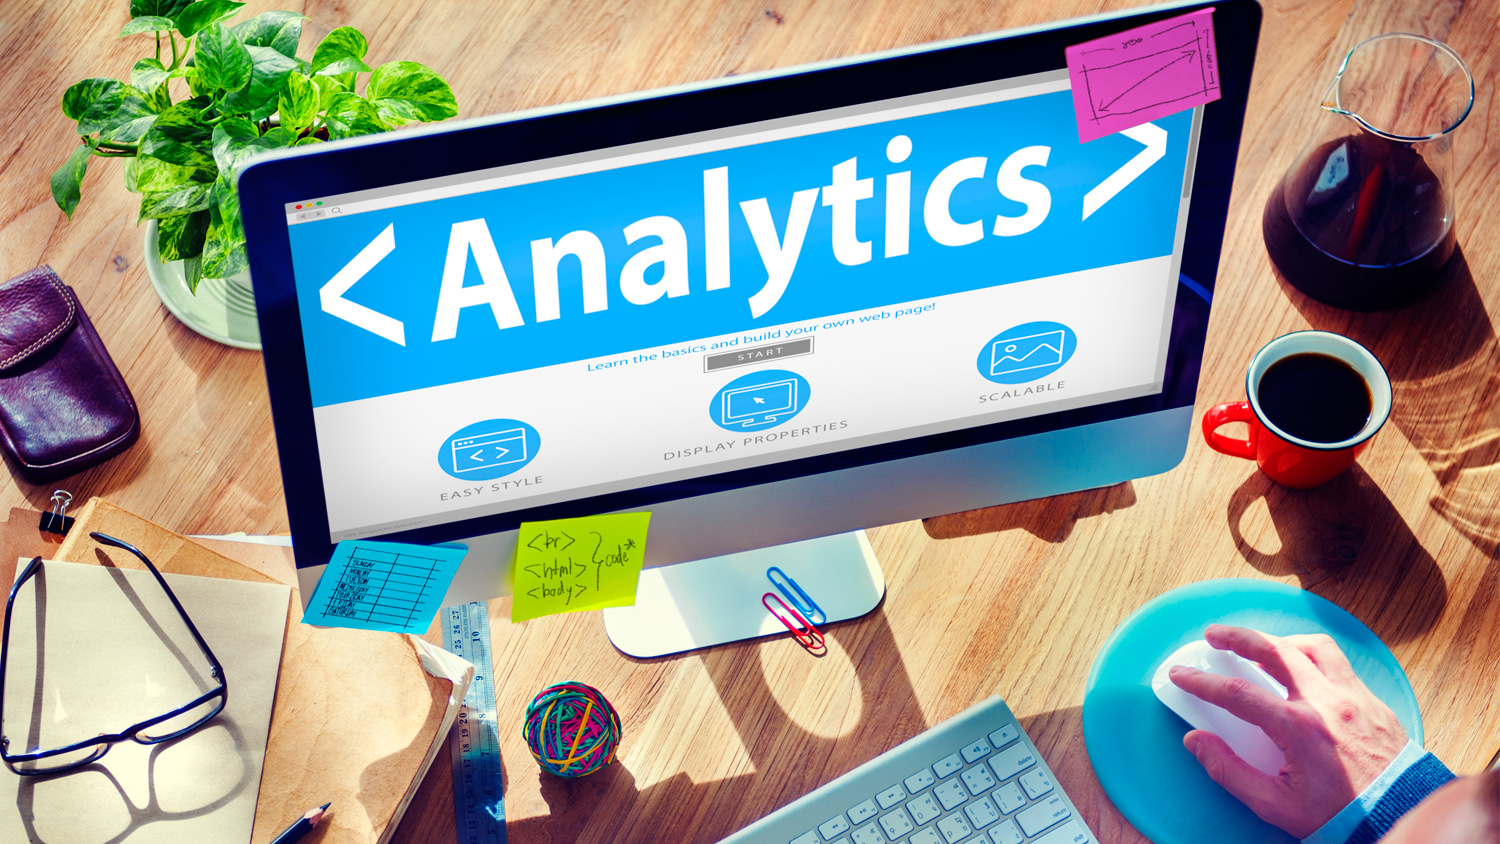
\includegraphics[width=14cm]{./images/foto1}\par\vspace{10cm}
\end{itemize}

El término Business Intelligence, también conocido como BI o Inteligencia empresarial, lleva más de 5 décadas en el diccionario de las empresas. Fue acuñado por primera vez a mediados de los años 60, con la introducción del concepto de base de datos y la necesidad de acumular de forma organizada información que podría ser útil para la empresa en la toma de decisiones.  En los últimos años, una nueva palabra ha surgido para dar mayor profundidad a este tema: Business Analytics. 

Marcar diferencias entre ambos conceptos no es una labor sencilla, porque los dos parten de un mismo principio: el aprovechamiento de la información para tomar mejores decisiones de negocios. Es más, muchos especialistas del tema optan por no puntuar diferencia alguna y más bien hablan de dos ideas que se complementan. Sin embargo, para otros teóricos, sí existen diferencias sutiles en cuanto a la naturaleza de la información recolectada y el modo en que esta es usada en beneficio de la empresa. En este artículo se abordará uno de los argumentos más utilizados en esta discusión, aunque vale mencionar que existen diversas aproximaciones del tema y no todas desembocan en la misma conclusión. 

El Business Intelligence nos permite echar un vistazo al pasado de la empresa a través de análisis y reportes que tienen como base información histórica del negocio. Es ideal para comprender el panorama de desarrollo histórico de una empresa. 

Por otro lado, el Business Analytics se enfoca en el análisis a futuro con base en la información de la empresa y modelos predictivos para apoyar la toma de decisiones y mejorar la competitividad del negocio. En otras palabras, el Business Analytics tiene un marcado enfoque en el análisis de la situación actual y la predicción de eventos futuros para entender el camino que tomará la empresa.

En síntesis, podemos entender el Business Intelligence como las formas de recolectar y entender datos del pasado, mientras que el Business Analytics nos permite construir una visión más clara del futuro. En todo caso, ambas herramientas pueden complementarse para elaborar un análisis detallado del funcionamiento y futuro de una empresa, con el fin de tomar mejores decisiones.

\subsection{Cómo abordar Business Intelligence y Business Analytics}
Para utilizar Business Intelligence y Business Analytics en beneficio de su empresa, primero debe determinar las métricas más importantes que su empresa necesita para medir y analizar con el fin de comprender la salud y el progreso actuales del negocio (en todos los departamentos), así como los puntos de referencia de negocios futuros.

Con una comprensión clara de los datos comerciales, y al recibir la aprobación ejecutiva en los puntos de datos delineados, podrá elaborar una guía común en toda la empresa para evaluar y evaluar las actividades comerciales. Con esta hoja de ruta, todos estarán en la misma página. El liderazgo empresarial puede aprovechar los conocimientos que proporcionan los datos y desarrollar estrategias empresariales productivas y planes de ejecución.    

La segunda pieza crucial de inteligencia de negocios y análisis de negocios es confiar en sus datos. No importa qué tan buenos sean sus datos, si su equipo o los líderes de su empresa no confían en él (y no lo utilizan como base para la toma de decisiones), la inteligencia empresarial y el análisis comercial no harán que su organización bueno. Un sistema de gestión de datos ágil y robusto que proporciona visualizaciones de datos fáciles de entender y capacidades de generación de informes es un componente esencial en la creación de confianza en los datos. Si su equipo confía en el sistema, confiarán en los datos que entrega.    

Pero encontrar el sistema adecuado puede ser una tarea desalentadora: con tantos sistemas diferentes de administración de datos, ¿cuál es el mejor para su empresa?

Ahí es donde entra en juego un socio de implementación como Hitachi Solutions. Ayudamos a nuestros clientes a identificar los datos que sus negocios necesitan, y luego desarrollamos e implementamos un sistema de administración de datos fácil de usar que cumple con sus requisitos y aumenta el crecimiento del negocio. Nuestros proyectos de análisis empresarial aprovechan Microsoft SQL Server BI , Azure Analytics , Cortana Intelligence Suite y Power BI , lo que nos permite crear potentes soluciones comerciales líderes en la industria.


\end{document}